\documentclass[11pt, a4paper]{article}  %(或book)
%\documentclass{emulateapj}
%\usepackage[Lenny]{fncychap}  %(章节的格式设置)
\usepackage{titlesec}
\titleformat{\section}{\Large\bfseries}{\thesection}{1em}{}
\titleformat{\subsection}{\large\bfseries}{\thesubsection}{1em}{}
% \titleformat{\section}{标题的格式,包括字体,字体大小,加粗}{标题序号,\thesection是数字,可自定义如“Di \thesection Zhang”}{标题序号与标题文字之间空格的大小,用pt或em,不能省}{标题文字大小,用\large等,可缺省}
\usepackage{amsmath}
\usepackage{amssymb}
\usepackage{float}
\usepackage{natbib}
\usepackage{color}
\usepackage{bm}
\usepackage{mathrsfs}
\usepackage{graphicx}
\usepackage{CJK}  %(CJK宏包,也可以写成\usepackage{CJKutf8})
\usepackage{setspace}
\usepackage{graphicx}
\usepackage{multirow}
\usepackage{tabularx}
\usepackage{indentfirst} % indent at each head of graphy
\usepackage{subfigure} % 在\begin{figure}环境下插入横排并列的子图
\usepackage{multicol} % 部分页面的文字分栏设置(不适用于图片和表格)
\usepackage[top=3cm, bottom=3cm, left=2cm, right=2cm]{geometry}  %(边距)
% \newgeometry{left=..} % 会另起一新页,然后从该新页开始使用新的边距,直到遇到 \restoregeometry 为止

\begin{document}
\begin{CJK}{UTF8}{gbsn}  %(用UTF8编码,否则可能乱码,一定要3个{}都有)
\nocite{*}
\setlength{\parskip}{6pt}  % 设置标题上下的间距(\setlenght要在\begin{document}之后才有效果)
\setlength{\baselineskip}{20pt} % 设置每一行的行距

%\begin{figure}[htbp]/[H]
%%\center
%\includegraphics[width=xxcm]{figure.eps}
%\subfigure{ \includegraphics[width=xxcm]{test1.eps} } % 注意\subfigure后有{}
%\subfigure{ \includegraphics[width=xxcm]{test2.eps} } % 插入横排并列图片
%\subfigure{ \includegraphics[width=xxcm]{test3.eps} }
%\caption{Explain of figure}
%\label{fig:figurelabel}
%\end{figure}

%\begin{table}[htbp]/[H]
%\center
%\begin{tabular}{llcccr}  % number of columns, c->center, l->left, r->right
%\hline\hline  % \hline->horizontal line
%& Mass($M_{\text{sun}}$) & Radius(km) \\  % use "&" to align, "$$" to insert formula, "\\" to break the row
%\label{tab:tablelabel}
%\end{tabular}
%\end{table}

%\begin{eqnarray}
%	f(t) = \left\{ \begin{aligned}
%			a+bt & \, \quad t<0 \\
%			0    & \, \quad t \ge 0
%\end{aligned} \right.
%\end{eqnarray}


\title{\huge Visibility相位校准公式 \bf }

\author{Qizhi Huang}
\date{\today}
\maketitle
%%%%%%%%%%%%%%% Begin %%%%%%%%%%%%%%%





\section{坐标系}

天球的XYZ坐标系:

\indent\indent +Z指向北天极,+X指向校准源所有赤经

地面的xyz坐标系:

\indent\indent +z指向天顶,+x指向当地的东方,+y指向当地的北方





\section{基线坐标变换}

地面上的基线坐标为$(x,y,z)$

xyz坐标系

(1)绕x轴转 $-(90-\text{lat})$ 度,此时+z指向+Z,+x指向+Y,+y指向-X

(2)再绕z轴转 $-90$ 度,此时+z指向+Z,+x指向+X,+y指向+Y

\begin{eqnarray}
	\begin{bmatrix} X_b \\ Y_b \\ Z_b \end{bmatrix}
		&=& \begin{bmatrix} \cos(-90) & \sin(-90) & 0 \\ -\sin(-90) & \cos(-90) & 0 \\ 0 & 0 & 1 \end{bmatrix} 
		    \begin{bmatrix} 1 & 0 & 0 \\ 0 & \cos(-90+\text{lat}) & \sin(-90+\text{lat}) \\ 0 & -\sin(-90+\text{lat}) & \cos(-90+\text{lat}) \end{bmatrix}
		    \begin{bmatrix} x \\ y \\ z \end{bmatrix} \nonumber \\
		&=& \begin{bmatrix} 0 & -1 & 0 \\ 1 & 0 & 0 \\ 0 & 0 & 1 \end{bmatrix} 
		    \begin{bmatrix} 1 & 0 & 0 \\ 0 & \sin(\text{lat}) & -\cos(\text{lat}) \\ 0 & \cos(\text{lat}) & \sin(\text{lat}) \end{bmatrix}
		    \begin{bmatrix} x \\ y \\ z \end{bmatrix} \nonumber \\ \nonumber \\
		&=& \begin{bmatrix} -y\sin(\text{lat})+z\cos(\text{lat}) \\ x \\ y\cos(\text{lat})+z\sin(\text{lat}) \end{bmatrix} 
\end{eqnarray}





\section{被观测纬度圈在天球上的坐标}

纬圈坐标 $(90-\text{Dec}, \varphi)$,其中$\varphi \Rightarrow \text{RA}$

由于+X指向校准源所有的赤经,于是校准源所在的 $\varphi_s=0$

\begin{equation}
	\begin{bmatrix} X_s \\ Y_s \\ Z_s \end{bmatrix}
		= \begin{bmatrix} \sin(90-\text{Dec})\cos(\varphi) \\ \sin(90-\text{Dec})\sin(\varphi) \\ \cos(90-\text{Dec}) \end{bmatrix}
		= \begin{bmatrix} \cos(\text{Dec})\cos(\varphi) \\ \cos(\text{Dec})\sin(\varphi) \\ \sin(\text{Dec}) \end{bmatrix} 
\end{equation}





\section{基线造成的相位延时}

\begin{eqnarray}
	\text{Phase} &=& \begin{bmatrix} X_b \\ Y_b \\ Z_b \end{bmatrix} \begin{bmatrix} X_s \\ Y_s \\ Z_s \end{bmatrix} \nonumber \\ 
		&=& x\cos(\text{Dec})\sin(\varphi) \nonumber \\
		&& + \, y\left[ \sin(\text{Dec})\cos(\text{lat}) - \cos(\text{Dec})\sin(\text{lat})\cos(\varphi) \right] \\
		&& + \, z\left[ \sin(\text{Dec})\sin(\text{lat}) + \cos(\text{Dec})\cos(\text{lat})\cos(\varphi) \right] \nonumber
\end{eqnarray}

当 $z=0$ 时:
\begin{equation}
	\text{Phase} = x\cos(\text{Dec})\sin(\varphi) + y\left[ \sin(\text{Dec})\cos(\text{lat}) - \cos(\text{Dec})\sin(\text{lat})\cos(\varphi) \right]
\end{equation}

当 $z=0$,$\varphi$ 是小角($\sin(\varphi) \approx \varphi$,$\cos(\varphi) \approx 1$)时:
\begin{eqnarray}
	\text{Phase} &\approx& x\cos(\text{Dec})\varphi + y\left[ \sin(\text{Dec})\cos(\text{lat}) - \cos(\text{Dec})\sin(\text{lat}) \right] \nonumber \\
		&=& x\cos(\text{Dec})\varphi + y\sin(\text{Dec}-\text{lat})
\end{eqnarray}




\section{纬圈上的波束(beam)}

一维高斯波束($\theta$ 从 $-$ 到 $0$ 再到 $+$):
\begin{equation} 
	\text{Beam} = \exp\left\{-\frac{\theta^2}{2\sigma^2}\right\}
\end{equation}

在天球坐标系XYZ中

\begin{equation}
	\begin{bmatrix} X_g \\ Y_g \\ Z_g \end{bmatrix}
		= \begin{bmatrix} \sin(90-\text{Dec})\cos(\varphi) \\ \sin(90-\text{Dec})\sin(\varphi) \\ \cos(90-\text{Dec}) \end{bmatrix}
		= \begin{bmatrix} \cos(\text{Dec})\cos(\varphi) \\ \cos(\text{Dec})\sin(\varphi) \\ \sin(\text{Dec}) \end{bmatrix} 
\end{equation}

将其旋转到被观测纬圈上:

\indent\indent 绕+X轴转 $90-\text{Dec}$ 度

\begin{eqnarray}
	\begin{bmatrix} x_g \\ y_g \\ z_g \end{bmatrix}
		&=& \begin{bmatrix} 1 & 0 & 0 \\ 0 & \cos(90-\text{Dec}) & \sin(90-\text{Dec}) \\ 0 & -\sin(90-\text{Dec}) & \cos(90-\text{Dec}) \end{bmatrix} \begin{bmatrix} X_g \\ Y_g \\ Z_g \end{bmatrix}
		= \begin{bmatrix} 1 & 0 & 0 \\ 0 & \sin(\text{Dec}) & \cos(\text{Dec}) \\ 0 & -\cos(\text{Dec}) & \sin(\text{Dec}) \end{bmatrix} \begin{bmatrix} X_g \\ Y_g \\ Z_g \end{bmatrix} \nonumber \\
		&=& \begin{bmatrix} \cos(\text{Dec})\cos(\varphi) \\ \sin(\text{Dec})\cos(\text{Dec})\sin(\varphi) + \sin(\text{Dec})\cos(\text{Dec}) \\ -\cos^2(\text{Dec})\sin(\varphi) + \sin^2(\text{Dec}) \end{bmatrix} \nonumber \\ \nonumber \\
		&=& \begin{bmatrix} \cos(\text{Dec})\cos(\varphi) \\ \sin(\text{Dec})\cos(\text{Dec})\left[1 + \sin(\varphi)\right] \\ 1-\cos^2(\text{Dec})\left[1 + \sin(\varphi)\right] \end{bmatrix} 
		= \begin{bmatrix} \sin(\theta_g)\cos(\varphi_g) \\ \sin(\theta_g)\sin(\varphi_) \\ \cos(\theta_g) \end{bmatrix}
\end{eqnarray}

可求得:
\begin{equation}
	\theta_g = \arccos\left\{ 1 - \cos^2(\text{Dec}) \left[1 + \sin(\varphi) \right] \right\} \, , \qquad
	\theta_g(\text{center}) = \arccos\left\{ \sin^2(\text{Dec}) \right\}
\end{equation}

于是,在纬圈上的一维高斯波束为:
\begin{eqnarray} 
	\text{Beam} &=& \exp\left\{-\frac{\left[\theta_g - \theta_g(\text{center})\right]^2}{2\sigma^2}\right\} \nonumber \\
		&=& \exp\left\{ -\frac{\left[\,\, \arccos\left\{1-\cos^2(\text{Dec})\left[1+\sin(\varphi)\right]\right\} - \arccos\left\{\sin^2(\text{Dec})\right\} \,\,\right]^2}{2\sigma^2} \right\}
\end{eqnarray}

当 $\varphi$ 是小角($\sin(\varphi) \approx \varphi$,$\cos(\varphi) \approx 1$)时:
\begin{equation} 
	\text{Beam} = \exp\left\{-\frac{ \left[\,\, \cos(\text{Dec})\varphi \,\,\right]^2 }{2\sigma^2}\right\}
\end{equation}





\section{纬圈上的一维visibility近似公式}

\begin{eqnarray}
	\text{Visibility} &=& \text{Beam}\cdot\exp\left\{i\cdot\text{Phase}\right\} \nonumber \\
		&=& \exp\left\{ -\frac{\left[\,\, \arccos\left\{1-\cos^2(\text{Dec})\left[1+\sin(\varphi)\right]\right\} - \arccos\left\{\sin^2(\text{Dec})\right\} \,\,\right]^2}{2\sigma^2} \right\} \nonumber \\ 
		&& \bullet \exp\left\{ i\frac{2\pi}{\lambda}  \left\{\, x\cos(\text{Dec})\sin(\varphi) + y\left[ \sin(\text{Dec})\cos(\text{lat}) - \cos(\text{Dec})\sin(\text{lat})\cos(\varphi) \right] \,\right\} \right\} \nonumber \\ \\ 
		&=& \exp\left\{-\frac{ \left[\, \cos(\text{Dec})\sin(\varphi) \,\right]^2 }{2\sigma^2}\right\} \cdot \exp\left\{ i\frac{2\pi}{\lambda} \left[\,x\cos(\text{Dec})\sin(\varphi) + y\sin(\text{Dec}-\text{lat})\,\right] \right\} \\ %\nonumber \\
		&=& \exp\left\{-\frac{ \left[\, \cos(\text{Dec})\varphi \,\right]^2 }{2\sigma^2}\right\} \cdot \exp\left\{ i\frac{2\pi}{\lambda} \left[\,x\cos(\text{Dec})\varphi + y\sin(\text{Dec}-\text{lat})\,\right] \right\}
\end{eqnarray}



''vis\_formula`` below is
\begin{equation}
	\text{vis\_formula} = \exp\left\{-\frac{ \left[\, \cos(\text{Dec})\varphi \,\right]^2 }{2\sigma^2}\right\} \cdot \exp\left\{ {\color{red}{\bm{-}}} i\frac{2\pi}{\lambda} \left[\,x\cos(\text{Dec})\varphi {\color{red}{\bm{-}}} y\sin(\text{Dec}-\text{lat})\,\right] \right\}
\label{eq:vis_formula}
\end{equation}

Use equation (\ref{eq:vis_formula}) to calibrate the phase, then can use my map-making program to make the map.



\begin{figure}[H]
\center
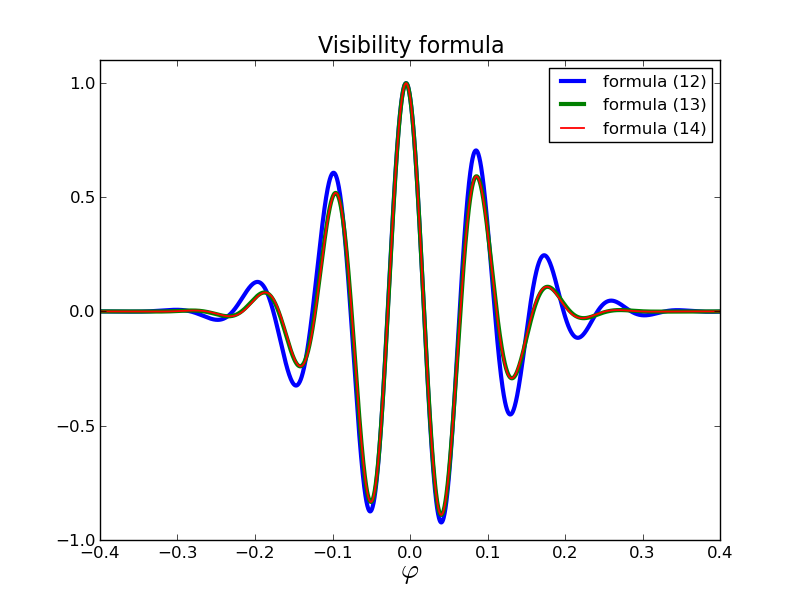
\includegraphics[width=8cm]{vis_formula.eps}
\end{figure}


\begin{figure}[H]
\subfigure{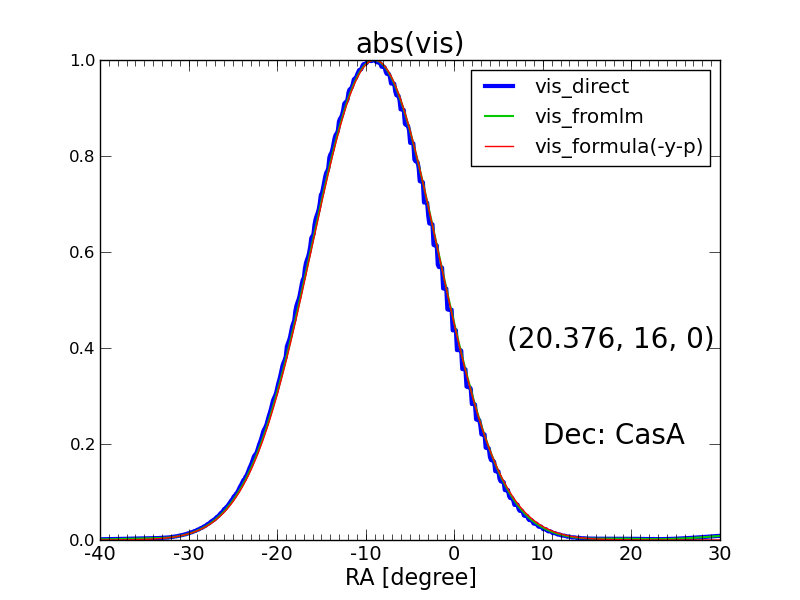
\includegraphics[width=8cm]{vis_direct-fromlm-formula_abs_-y-p_CasA_-2.eps}}
\subfigure{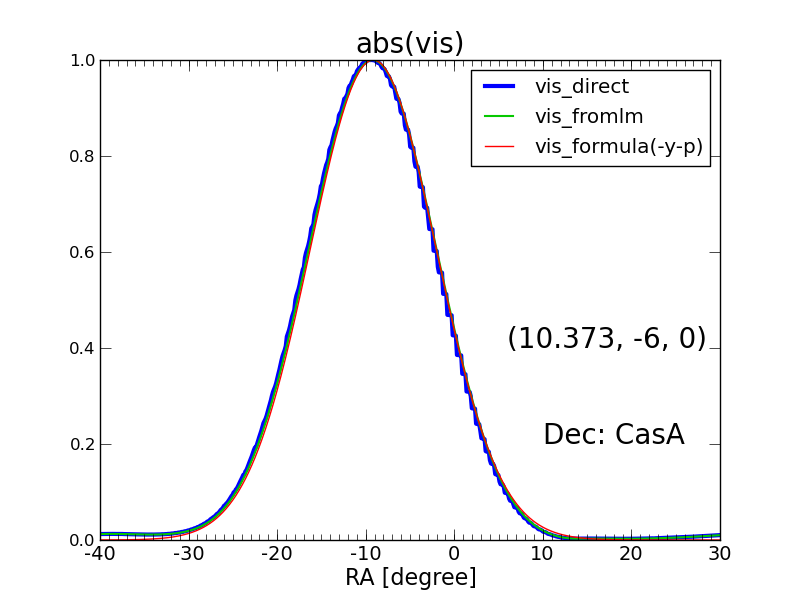
\includegraphics[width=8cm]{vis_direct-fromlm-formula_abs_-y-p_CasA_-3.eps}}
\end{figure}
\begin{figure}[H]
\subfigure{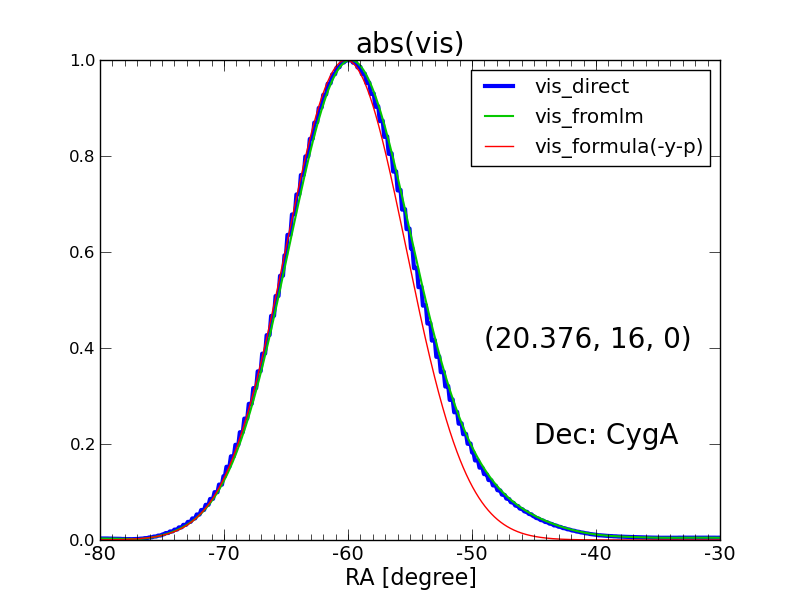
\includegraphics[width=8cm]{vis_direct-fromlm-formula_abs_-y-p_CygA_-2.eps}}
\subfigure{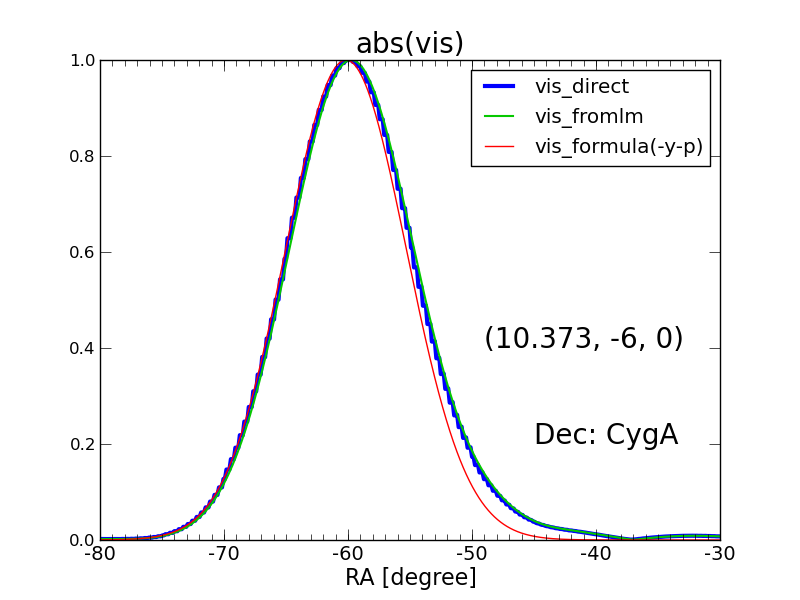
\includegraphics[width=8cm]{vis_direct-fromlm-formula_abs_-y-p_CygA_-3.eps}}
\end{figure}

\begin{figure}[H]
\subfigure{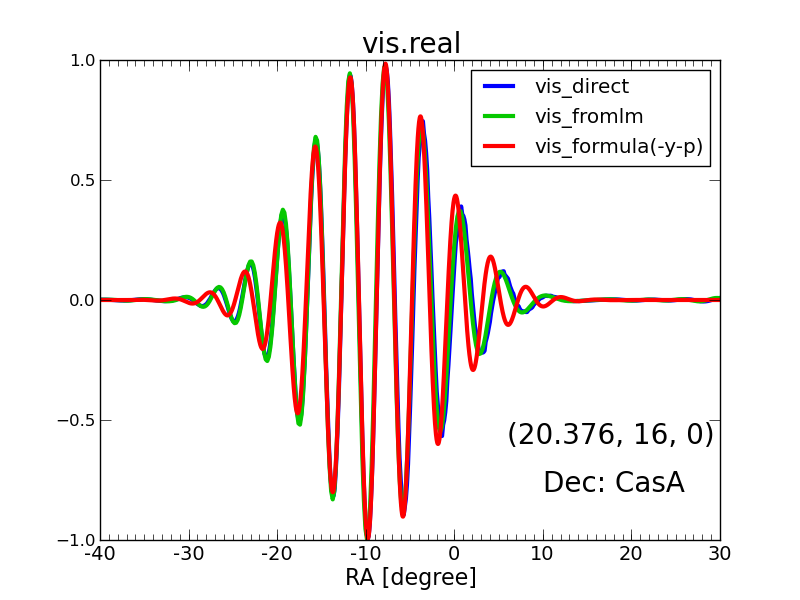
\includegraphics[width=8cm]{vis_direct-fromlm-formula_real_-y-p_CasA_-2.eps}}
\subfigure{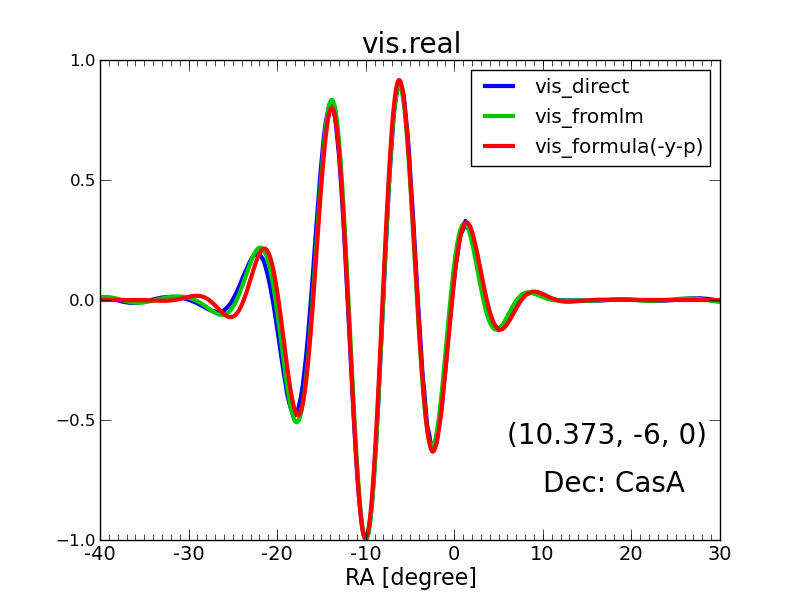
\includegraphics[width=8cm]{vis_direct-fromlm-formula_real_-y-p_CasA_-3.eps}}
\end{figure}
\begin{figure}[H]
\subfigure{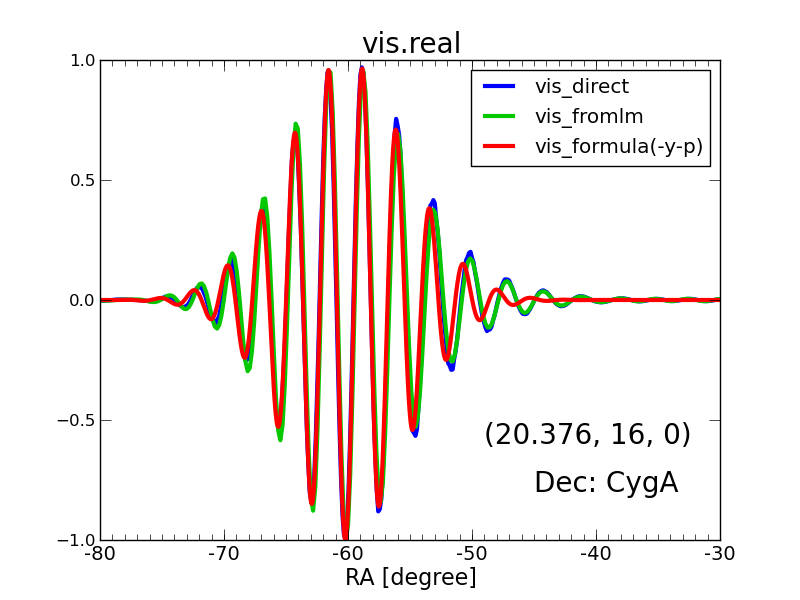
\includegraphics[width=8cm]{vis_direct-fromlm-formula_real_-y-p_CygA_-2.eps}}
\subfigure{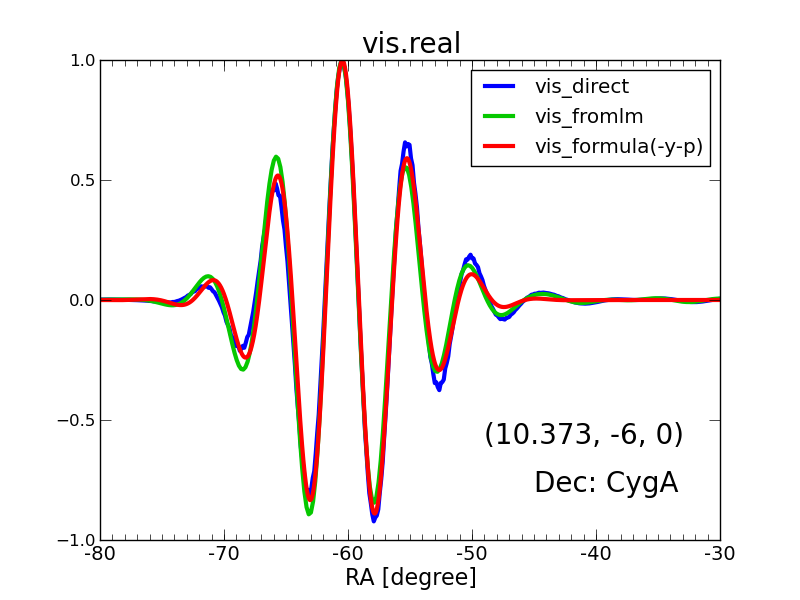
\includegraphics[width=8cm]{vis_direct-fromlm-formula_real_-y-p_CygA_-3.eps}}
\end{figure}

\begin{figure}[H]
\subfigure{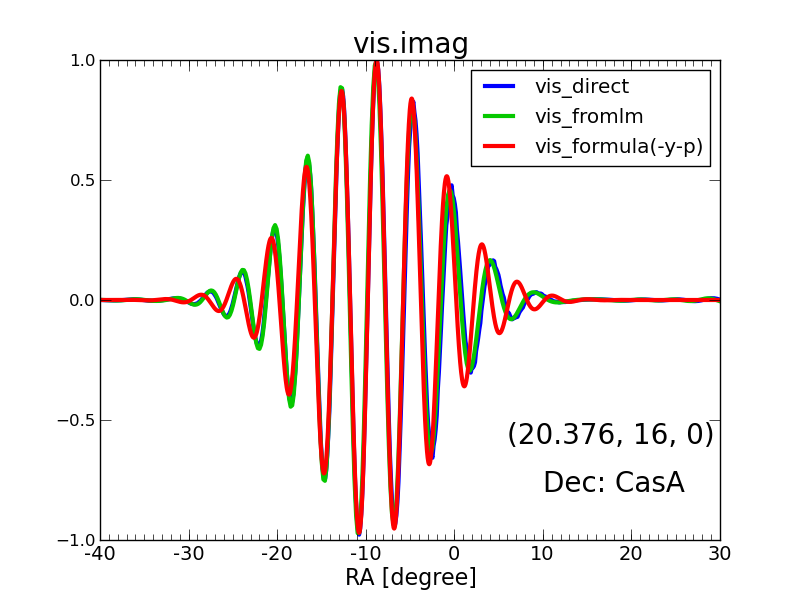
\includegraphics[width=8cm]{vis_direct-fromlm-formula_imag_-y-p_CasA_-2.eps}}
\subfigure{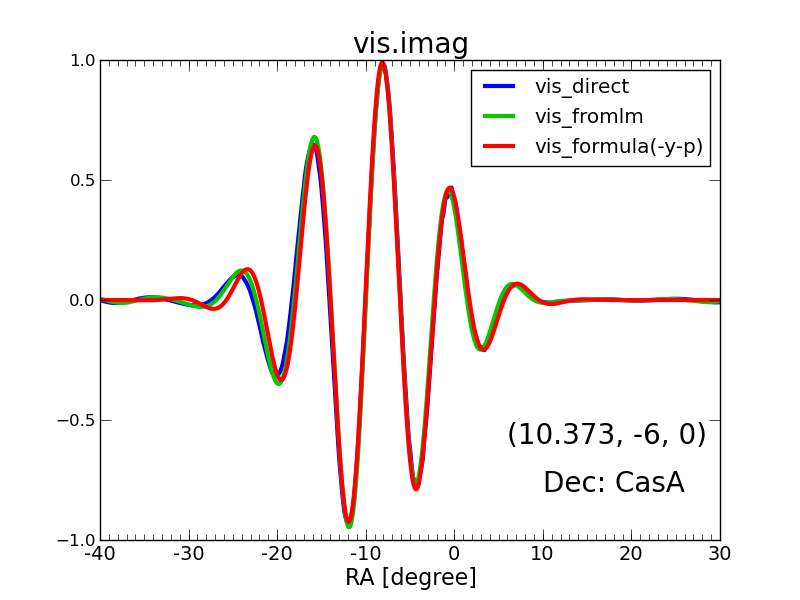
\includegraphics[width=8cm]{vis_direct-fromlm-formula_imag_-y-p_CasA_-3.eps}}
\end{figure}
\begin{figure}[H]
\subfigure{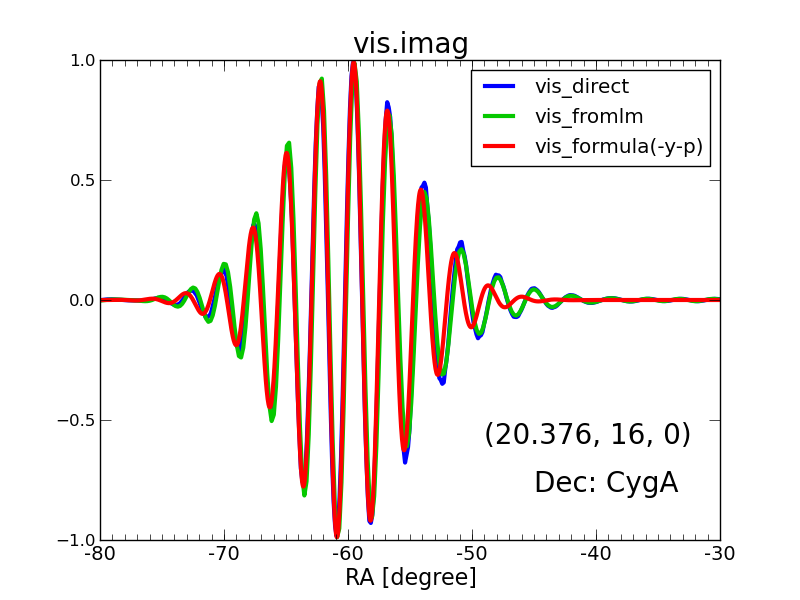
\includegraphics[width=8cm]{vis_direct-fromlm-formula_imag_-y-p_CygA_-2.eps}}
\subfigure{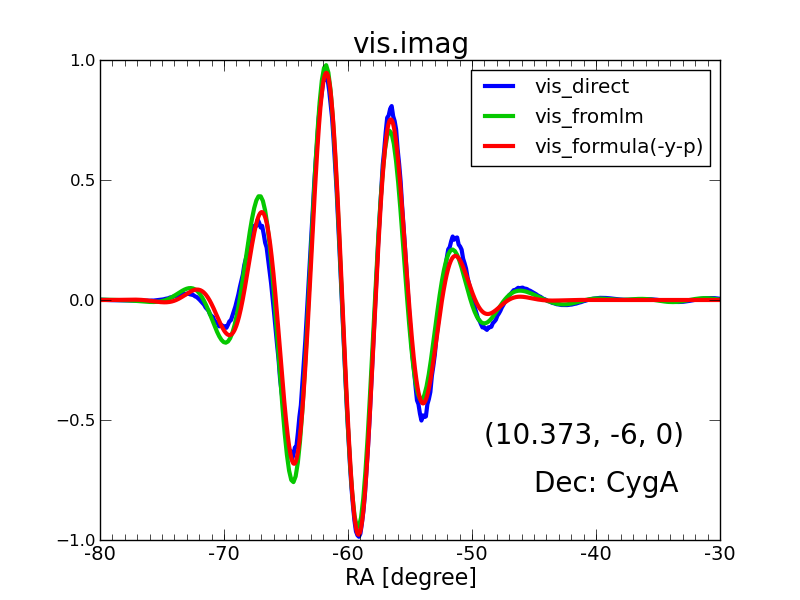
\includegraphics[width=8cm]{vis_direct-fromlm-formula_imag_-y-p_CygA_-3.eps}}
\end{figure}



%%%%%%%%%%%%%%% End %%%%%%%%%%%%%%%
\end{CJK}
\end{document}
